% Options for packages loaded elsewhere
\PassOptionsToPackage{unicode}{hyperref}
\PassOptionsToPackage{hyphens}{url}
%
\documentclass[
  british,
  man,floatsintext]{apa6}
\usepackage{lmodern}
\usepackage{amssymb,amsmath}
\usepackage{ifxetex,ifluatex}
\ifnum 0\ifxetex 1\fi\ifluatex 1\fi=0 % if pdftex
  \usepackage[T1]{fontenc}
  \usepackage[utf8]{inputenc}
  \usepackage{textcomp} % provide euro and other symbols
\else % if luatex or xetex
  \usepackage{unicode-math}
  \defaultfontfeatures{Scale=MatchLowercase}
  \defaultfontfeatures[\rmfamily]{Ligatures=TeX,Scale=1}
\fi
% Use upquote if available, for straight quotes in verbatim environments
\IfFileExists{upquote.sty}{\usepackage{upquote}}{}
\IfFileExists{microtype.sty}{% use microtype if available
  \usepackage[]{microtype}
  \UseMicrotypeSet[protrusion]{basicmath} % disable protrusion for tt fonts
}{}
\makeatletter
\@ifundefined{KOMAClassName}{% if non-KOMA class
  \IfFileExists{parskip.sty}{%
    \usepackage{parskip}
  }{% else
    \setlength{\parindent}{0pt}
    \setlength{\parskip}{6pt plus 2pt minus 1pt}}
}{% if KOMA class
  \KOMAoptions{parskip=half}}
\makeatother
\usepackage{xcolor}
\IfFileExists{xurl.sty}{\usepackage{xurl}}{} % add URL line breaks if available
\IfFileExists{bookmark.sty}{\usepackage{bookmark}}{\usepackage{hyperref}}
\hypersetup{
  pdftitle={Studying behaviour change mechanisms under complexity},
  pdfkeywords={complex systems, wellbeing, methodology, behaviour change},
  hidelinks,
  pdfcreator={LaTeX via pandoc}}
\urlstyle{same} % disable monospaced font for URLs
\usepackage{graphicx,grffile}
\makeatletter
\def\maxwidth{\ifdim\Gin@nat@width>\linewidth\linewidth\else\Gin@nat@width\fi}
\def\maxheight{\ifdim\Gin@nat@height>\textheight\textheight\else\Gin@nat@height\fi}
\makeatother
% Scale images if necessary, so that they will not overflow the page
% margins by default, and it is still possible to overwrite the defaults
% using explicit options in \includegraphics[width, height, ...]{}
\setkeys{Gin}{width=\maxwidth,height=\maxheight,keepaspectratio}
% Set default figure placement to htbp
\makeatletter
\def\fps@figure{htbp}
\makeatother
\setlength{\emergencystretch}{3em} % prevent overfull lines
\providecommand{\tightlist}{%
  \setlength{\itemsep}{0pt}\setlength{\parskip}{0pt}}
\setcounter{secnumdepth}{-\maxdimen} % remove section numbering
% Make \paragraph and \subparagraph free-standing
\ifx\paragraph\undefined\else
  \let\oldparagraph\paragraph
  \renewcommand{\paragraph}[1]{\oldparagraph{#1}\mbox{}}
\fi
\ifx\subparagraph\undefined\else
  \let\oldsubparagraph\subparagraph
  \renewcommand{\subparagraph}[1]{\oldsubparagraph{#1}\mbox{}}
\fi
% Manuscript styling
\usepackage{upgreek}
\captionsetup{font=singlespacing,justification=justified}

% Table formatting
\usepackage{longtable}
\usepackage{lscape}
% \usepackage[counterclockwise]{rotating}   % Landscape page setup for large tables
\usepackage{multirow}		% Table styling
\usepackage{tabularx}		% Control Column width
\usepackage[flushleft]{threeparttable}	% Allows for three part tables with a specified notes section
\usepackage{threeparttablex}            % Lets threeparttable work with longtable

% Create new environments so endfloat can handle them
% \newenvironment{ltable}
%   {\begin{landscape}\begin{center}\begin{threeparttable}}
%   {\end{threeparttable}\end{center}\end{landscape}}
\newenvironment{lltable}{\begin{landscape}\begin{center}\begin{ThreePartTable}}{\end{ThreePartTable}\end{center}\end{landscape}}

% Enables adjusting longtable caption width to table width
% Solution found at http://golatex.de/longtable-mit-caption-so-breit-wie-die-tabelle-t15767.html
\makeatletter
\newcommand\LastLTentrywidth{1em}
\newlength\longtablewidth
\setlength{\longtablewidth}{1in}
\newcommand{\getlongtablewidth}{\begingroup \ifcsname LT@\roman{LT@tables}\endcsname \global\longtablewidth=0pt \renewcommand{\LT@entry}[2]{\global\advance\longtablewidth by ##2\relax\gdef\LastLTentrywidth{##2}}\@nameuse{LT@\roman{LT@tables}} \fi \endgroup}

% \setlength{\parindent}{0.5in}
% \setlength{\parskip}{0pt plus 0pt minus 0pt}

% \usepackage{etoolbox}
\makeatletter
\patchcmd{\HyOrg@maketitle}
  {\section{\normalfont\normalsize\abstractname}}
  {\section*{\normalfont\normalsize\abstractname}}
  {}{\typeout{Failed to patch abstract.}}
\makeatother
\shorttitle{Complexity in behaviour change mechanisms}
\author{Matti T. J. Heino\textsuperscript{1}, Keegan Knittle\textsuperscript{1}, Chris Noone\textsuperscript{2}, Fred Hasselman\textsuperscript{3}, \& Nelli Hankonen\textsuperscript{1}}
\affiliation{
\vspace{0.5cm}
\textsuperscript{1} Faculty of Social Sciences, University of Helsinki, PO Box 54, 00014 University of Helsinki, Finland\\\textsuperscript{2} \\\textsuperscript{3} }
\authornote{

Correspondence concerning this article should be addressed to Matti T. J. Heino, Faculty of Social Sciences, University of Helsinki, PO Box 54, 00014 University of Helsinki, Finland. E-mail: matti.tj.heino@gmail.com}
\note{This is a preprint submitted for publication}
\keywords{complex systems, wellbeing, methodology, behaviour change}
\usepackage{lineno}

\linenumbers
\usepackage{csquotes}
\usepackage{booktabs}
\usepackage{float}
\usepackage{setspace}
\AtBeginEnvironment{tabular}{\singlespacing}
\AtBeginEnvironment{lltable}{\singlespacing}
\AtBeginEnvironment{tablenotes}{\doublespacing}
\captionsetup[table]{font={stretch=1.5}}
\captionsetup[figure]{font={stretch=1.5}}
\ifxetex
  % Load polyglossia as late as possible: uses bidi with RTL langages (e.g. Hebrew, Arabic)
  \usepackage{polyglossia}
  \setmainlanguage[variant=british]{english}
\else
  \usepackage[shorthands=off,main=british]{babel}
\fi

\title{Studying behaviour change mechanisms under complexity}

\date{}

\abstract{
Knowledge of how behaviour changes, i.e.~the mechanisms underlying the effects of behaviour change interventions, is vital for accumulating valid scientific evidence and informing practice and policy-making across multiple domains. Traditional approaches to such evaluations have applied study designs and statistical models which implicitly assume that change is linear, constant and caused by independent influences on behaviour (such as behaviour change techniques), despite the theories' somewhat more elaborate accounts of these relationships. This article illustrates limitations of these standard statistical tools, and considers the benefits of adopting a complex adaptive systems approach to behaviour change research.

This paper will 1) outline the sometimes-overlooked complexity of behaviours and behaviour change interventions, 2) introduce readers to some key features of complex systems and how these relate to human behaviour change, and 3) provide suggestions for how researchers can better account for implications of complexity in analysing change mechanisms. We focus on three common features of complex systems (i.e.~interconnectedness, non-ergodicity and non-linearity), and introduce recurrence quantification analysis, a method able to deal with data data stemming from a system with these features. The supplemental website {[}link xxx{]} provides exemplifying code and data for practical analysis applications. The complex adaptive systems approach offers a host of novel computational methods and opens novel avenues for understanding and theorising about the dynamics of behaviour change.
}

\begin{document}
\maketitle

\newpage

\hypertarget{introduction}{%
\section{Introduction}\label{introduction}}

In order to understand why behavioural interventions often fail to produce sustainable effects (Kwasnicka et al., 2016), especially when transferred from one context to another, a core interest of behaviour change science is to improve our understanding of mechanisms of behaviour change. Behavioural theories identify hundreds of potential \enquote{determinants} of behaviour, that is, factors that potentially influence the behaviour of interest, constituting the mechanisms by which behaviour change techniques might influence behaviour (Carey et al., 2019). These range from cognitions such as self-efficacy and attitudes, to biological factors, and certain elements of the social and built environments in which behaviours take place (Michie et al., 2014). When studied using typical linear designs and statistical models, the relationships between causal precedents and behaviour change are assumed to be simple, constant and linear (i.e.~the outputs are proportional to the inputs). However, it is our position that this offers behaviour change researchers and the general public an inaccurate or at least imprecise understanding of behaviour change. New paradigms are needed, which consider the relevant factors as complex, potentially non-linear, and oft-changing.

The evaluation of behaviour change interventions typically involves randomly assigning participants to receive an intervention of interest or a specific comparator and measuring subjective and objective indicators of behaviour. Usually, these measurements occur immediately before and after the delivery of the intervention, though sometimes additional follow-up measurements may take place weeks or months later. This is the classic Randomised Controlled Trial design and the data produced are most often analysed using statistical techniques that are specific cases of the General Linear Model. We refer to this as the conventional approach in this paper. If the interest is only in assessing whether the treatment overall was more effective, on average, in the intervention group than the control group, comparing averages in randomised controlled trials can be purposeful and acceptable (i.e.~answering questions such as \enquote{Does the intervention have an effect on the target behaviour?}, \enquote{Do cohorts differ from each other?}). However, studying behaviour change mechanisms (\enquote{How do intervention participants change?}) with few measurement points only, results in problems. Limiting the study of behaviour change dynamics in that way, also limits our understanding of how changes occur under different conditions over time. Recently, solutions stemming from complex systems science (Siegenfeld \& Bar-Yam, 2019) have become increasingly accessible and helpful in tackling problems of understanding change processes.

While a reliance on linear models simplifies the analytical approaches needed to explore relationships between variables, it does not contribute to our understanding of how the world works, as \enquote{most of everyday life is nonlinear} (Strogatz, 2018, p. 9) and outside the physical sciences, nonlinear systems are \enquote{the rule, not the exception} (May, 1976, p. 467). As an intuitive example, consider that falling from 10 meters is likely to kill you, but falling from one meter does not make you 1/10th dead -- in fact, it makes you stronger (Taleb, 2013, 2012). Or that eating twice the size of a normal meal rarely results in twice the pleasure. Human behaviour is complex, and while we have formulated theoretical constructs to be as amenable as possible to linear methods of analysis, this may obscure important characteristics of behaviour change. This paper will 1) outline the sometimes-overlooked complexity of behaviours and behaviour change interventions, 2) introduce readers to some key features of complex systems and how these can be applied to human behaviour, and 3) provide concrete suggestions for how researchers can better account for the implications of complexity in analysing behaviour change mechanisms.

\hypertarget{what-are-complex-systems}{%
\subsection{What are complex systems?}\label{what-are-complex-systems}}

A system is \enquote{a delineated part of the universe which is distinguished from the rest by an imaginary boundary} (Bar-Yam, 2018), although other definitions exist (see Wright \& Meadows, 2009 for a primer). Many things - a central nervous system, a school, a community, a society - can be conceptualised as systems (or interacting levels of a single system). This paper focuses on individual people as complex systems. Complex systems can be characterised as webs of many interdependent self-organising parts that operate without central control, whose interactions give rise to emergent properties and behaviours (Mitchell, 2009). Individual persons or other system components contribute and adapt to each others' environments, coevolving with each other to create macro-level behaviour, which is difficult to predict and usually not changeable in a stepwise engineering sense (Brand et al., 2015). These characteristics distinguish complex systems from those which are just complicated: Highly complicated processes or systems (e.g.~an airplane), unlike complex ones (e.g.~the brain) cannot, for example, self-organise to function adaptively when a part is removed (Rickles et al., 2007). Guides to basic terminology of chaos and complexity for scientists working with health behaviours can be found in Rickles, Hawe and Shiell (2007) as well as table 1 of Brand et al.~(2015).

\hypertarget{the-relevance-of-complexity-for-behaviour-change}{%
\subsection{The relevance of complexity for behaviour change}\label{the-relevance-of-complexity-for-behaviour-change}}

To paint a picture of just how complex the behavioural world is, take the case of physical activity as an example behaviour. Already three and a half decades ago, more than 30 influences on (or \enquote{determinants of}) this behaviour were being considered, along with calls for better understanding of their dynamics, interactions, and the time scales over which these develop (Dishman et al., 1985). While any influence (e.g.~intention, attitude) could have a direct relationship with physical activity, some rely on interactions with other influences to affect behaviour (e.g.~preventive behaviours being dependent on fear only in the presence of sufficient efficacy beliefs; (Kok et al., 2018; Peters et al., 2018). Furthermore, these interactions may be moderated by additional factors, and by other variables which themselves have no direct relationship with physical activity, with synergistic and opposing effects which may themselves depend on whether some threshold is exceeded. The extent to which all known (and unknown) influences on physical activity interact with one another presents a map of practically infinite, intertwined \enquote{routes} to initiating and maintaining the activity.

As mentioned above, evaluations of behaviour change interventions tend to focus on whether change occurs, while neglecting a focus on how behaviour changes. In attempts to understand how physical activity changes, the role of time brings added complexity to this behavioural world, as patterns of activity change over time and at varying frequencies. For example, fluctuations clearly occur within a day, as most individuals are (at least in the absence of highly sedentary working conditions and considerable somnambulism) more active while awake than while asleep. Fluctuation also occurs over the course of a week, as activity levels tend to be higher on weekdays than on weekends (Matthews et al., 2002); over the course of months, as activity levels are higher in warmer seasons and lower in colder ones (Cepeda et al., 2018); and over the course of years, as activity levels tend to decline with age (Dumith et al., 2011).

While we know something about how physical activity fluctuates over time, we know considerably less about how influences of behaviour change over time, and next to nothing about how the interactions of the influences fluctuate over time. We therefore also do not know how the fluctuations of interactions of influences interact with naturally occurring fluctuations in behaviour, or about the necessary preconditions for interactions between fluctuations in either influences or behaviour. It seems reasonable that, in addition to being dependent on their own past values, influences on behaviour are also affected by the past values of other variables, likely over various distances in times (i.e.~time lags). Furthermore, while much of our knowledge about the behavioural world was built on the assumption that relationships between variables are reasonably approximated as linear, we cannot rule out that relationships amongst these variables could substantially better described as e.g.~curvilinear, sigmoid or chaotic.

Therefore, as said above, the conventional approach of using linear models to assess behaviour change over very few time points limits the types of research questions we can ask about how behavioural changes occur. Why are linear models inappropriate for many of our research questions in the behavioural sciences? First, with many nonlinear interactions across time scales, our simplistic notions of causality (including mediation and moderation) might become deficient at best (Richardson et al., 2017; Rickles, 2009). Second, traditional statistical analyses may lead us astray, as there are enough potential context-dependent patterns to be \enquote{analogous to higher order interaction terms that could involve 5, 10, or 15-way interactions} in linear models (Resnicow \& Vaughan, 2006) -- everything depends on everything else, contributing what Meehl (1990, p. 204) coined as \enquote{the crud factor}. This also means a violation of the assumptions regarding independence and interference (Fink et al., 2016; Wallot \& Kelty-Stephen, 2017). Finally, forecasting in complex systems is notoriously difficult (Makridakis et al., 2019; Makridakis \& Taleb, 2009), making hypothesis testing---which is, after all, the test of a prediction---in intervention evaluation a curious challenge, one which will require behavioural scientists to familiarise themselves with complexity science (Rickles, 2009; Siegenfeld \& Bar-Yam, 2019). This is because a linear analysis will only give results that are correct given the assumption that the components in the model are independent, with additive effects that can be decomposed and attributed to their causes (e.g.~beta coefficients in multiple regression). If, on the other hand, these \enquote{component-dominant} dynamics are not driving the system, but instead the effects are intertwined, overlapping and inseparable (as proposed in the health context by Peters and Crutzen (2017)), and thus the dynamics are \enquote{interaction-dominant}, then replication and generalisation issues for results stemming from the linear analysis are almost inevitable (Wallot \& Kelty-Stephen, 2017).

Next, we describe some key concepts in systems science and highlight the challenges which a complex systems ontology presents for the assumptions inherent in traditional theorising and statistical models. Complex adaptive systems in the behaviour change research context have been previously discussed by Gomersall (2018), with a focus on simulation and qualitative methods. We complement this contribution by providing candidate quantitative modelling solutions to investigate behavior change phenomena with a complex systems lens.

\hypertarget{implications-for-behaviour-change-interventions}{%
\subsection{Implications for behaviour change interventions}\label{implications-for-behaviour-change-interventions}}

Although behaviour change maintenance has been theorised at length (Kwasnicka et al., 2016), systems science perspectives have been missing from this work. The effects of behaviour change interventions can be considered as shocks to the system in which they take place -- the aim of the shock is to alter the system's status, pushing against existing forces to affect change (Hawe et al., 2009; Olthof, Hasselman, Strunk, Aas, et al., 2019). This is akin to attempts to work against gravity, which pulls a ball in a valley (a relatively stable state, also known as an attractor; see figure \ref{fig:ballvalley}) to the bottom of it. Taking the analogy further, pushing the ball outside of the valley may lead it to roll off a peak, ending up in a deeper valley (i.e.~more dysfunctional state) than from where it started. A complex systems perspective implies, that even in the event of a successful intervention, stabilizing a system in a more functional state may require at least as many resources as the initial change itself (Bar-Yam, 2004, p. 211). In general, while complex systems may often be impossible to control precisely, they can be stewarded approximately, while allowing for variability stemming from self-organisation to flourish instead of trying to iron it out (Navarro \& Rueff-Lopes, 2015; Taleb \& Blyth, 2011). The necessity of complex systems approach is increasingly recognized. For example, it is highlighted in the UK Medical Research Council's recently updated guidance for development and evaluation of complex interventions (Skivington et al., 2018).

\begin{figure}
\centering
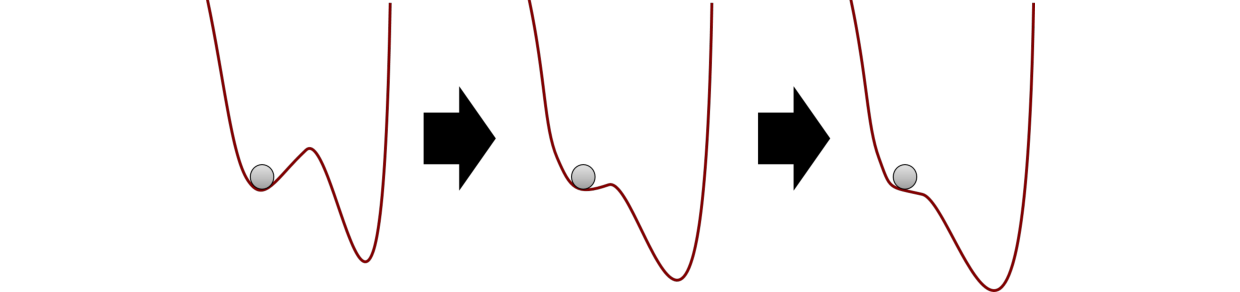
\includegraphics{_complexity-manuscript_files/figure-latex/ballvalley-1.pdf}
\caption{\label{fig:ballvalley}Evolution in attractor landscape: An intervention moulds a system, making it less stable, hence easier for the ball to move from current state (left) to another one (right).}
\end{figure}

Having now undergone a brief conceptual introduction to complexity, we can adapt Wright and Woods (2020) and define behaviour change as \emph{a collection of contextualised processes, that are nontrivially specific to each individual, forming a complex interconnected system, which is not restricted to linear dynamics}. We highlight three features of this definition:

\begin{enumerate}
\def\labelenumi{\arabic{enumi}.}
\tightlist
\item
  A complex interconnected system: There is a multitude of variables and timescales, which are interweaved, interdependent, and interacting.
\item
  Contextualised processes, specific to each individual: Individuals follow meaningfully different change trajectories, and develop, that is, change with time.
\item
  Not restricted to linear dynamics: Inputs are not necessarily proportional to outputs, and long periods of apparent stability can be followed with short periods of rapid change.
\end{enumerate}

\hypertarget{behaviour-change-mechanisms-under-complexity-three-key-features}{%
\section{Behaviour change mechanisms under complexity: Three key features}\label{behaviour-change-mechanisms-under-complexity-three-key-features}}

In the following three sections, we drill further down into these ideas. In the first, we introduce interaction-dominant dynamics, which flow from point 1 above; second, we present how idiosyncratic, non-stationary change trajectories lead to non-ergodicity, a technical term for the 2nd point; third, we highlight that the flexibility of complex systems leads to ubiquitous nonlinear processes as alluded to in point 3. Table 1 provides an overview of these ideas.

\textless\textless{} Insert Table 1 about here \textgreater\textgreater{}

\begin{table}[tbp]

\begin{center}
\begin{threeparttable}

\caption{\label{tab:summary-table}Main ideas presented in this manuscript.}

\begin{tabular}{llll}
\toprule
  & \multicolumn{1}{c}{Interconnectedness} & \multicolumn{1}{c}{Non-ergodicity} & \multicolumn{1}{c}{Non-linear dynamics}\\
\midrule
Description & The structure of a system---how it is organised and the relationships between its component parts---can matter more than the component parts themselves. Includes interconnectedness of different variables such as attitudes or perceived norms, as well as that of their temporal dependence; dynamic dependencies of complex systems are not restricted to one or a few previous time points. & A process is ergodic, when it is stationary, and all individuals in the population follow the same dynamics. Although required to infer within-individual processes from between-individual data, it is implausible for most psychological phenomena to display ergodicity, which has also been shown empirically, pointing to a threat to validity stemming from lack of group-to-individual generalisability for many areas of science. & In a linear progression of a phenomenon, the whole is exactly the sum of its parts: You can calculate how much each influencer of behaviour changes, and add them together to get the total effect. Non-linearity occurs when a systems’s inputs are disproportionate to its outputs. For example, an effect might be imperceptible for a long time, then explode (as in exponential growth), or suddenly switch states upon reaching a threshold.\\
Main lesson & Dynamic, intertwined processes do not exist in a vacuum, but are always co-dependent and cannot be partialed out into variance components without losing essential information on how the system as a whole operates. & Avoid the ecological fallacy (i.e., making individual-level inferences from group-level data) and thereby avoid misleading or incorrect inferences regarding individual behaviour. & Viewing the world solely from the lens of linear phenomena and relationships, leads to missed opportunities and misunderstood impacts of interventions.\\
Recommendations for the research community & Moving traditional regression-based approaches, which are inspired by component-dominant, additive dynamics (that the effects, or beta coefficients, of each variable can be summed together), linear approximations and Gaussian distributions, to methods able to cope with multiplicative effects and thick-tailed distributions. & Moving from large-sample research with many variables and many people but few time points (one model per sample), to N-of-1 and time series designs, with usually less people and less variables, but more data per variable (one model per individual). & Moving from linear approximations with the illusion of predictability, to methods which can accommodate non-linear patterns and disproportionate influences.\\
Useful resources & @richardsonInteractionDominantDynamicsTimescale2017; @wallotInteractionDominantCausationMind2017; @vanrooijFractalApproachDynamic2013 & @fisherLackGrouptoindividualGeneralizability2018; @molenaarImplicationsClassicalErgodic2008; @petersErgodicityProblemEconomics2019 & @helmichSuddenGainsDaytoday2020; @kelty-stephenMultifractalityMonoFractality2017; @westHomeostasisGaussStatistics2010\\
\bottomrule
\end{tabular}

\end{threeparttable}
\end{center}

\end{table}

\hypertarget{interconnectedness}{%
\subsection{Interconnectedness}\label{interconnectedness}}

When processes in complex systems are not independent, they are said to be coupled. Coupling can be unidirectional (where, for example, physical activity increases muscle mass but not the other way around), or bidirectional, where the elements of a system (e.g.~good performance and rewards) simultaneously reinforce or suppress each other as time progresses, demonstrating a type of circular causality. As alluded to earlier, dynamics in living systems tend to be dominated by synergies (\enquote{interaction-dominant causation}) instead of their component parts (\enquote{component-dominant causation}) (Bak et al., 1987; Richardson et al., 2017; Wallot \& Kelty-Stephen, 2017). Many psychological and behaviour change theories seem to at least implicitly assume the presence of reciprocal causation and intertwined processes (e.g.~Bandura, 1986, p. 6), but empirical testing of such processes has to date been limited.

Within the conventional approach to behaviour change intervention evaluation, researchers commonly employ mediation analyses to examine mechanisms. However, the clean \emph{independent variable} -\textgreater{} \emph{mediator} -\textgreater{} \emph{dependent variable} type of path analysis can be misleading, when change is in fact driven by self-reinforcing interactions. In component-dominant causation, effects follow causes in this type of a billiard-ball fashion, and one variable can change without everything else changing. For example, a study developed with the component-dominant mindset could aim to find out how using a specific behaviour change technique, say goal setting, affects behaviour. On the other hand, variables of interest to behaviour change researchers are unlikely to change without affecting a large amount of other, related variables (Peters \& Crutzen, 2017), producing highly context-dependent effects (Craig et al., 2018). This, too, implies that interaction-dominant causation is a more plausible framework for the behaviour change domain, wherein effects emerge (and are conditional upon) the system's holistic multivariate dynamics, with everything potentially taking place simultaneously in a circularly causal manner. Importantly, the interactions take place not just between variables, but also their temporal dynamics: Processes taking place on fast timescales (e.g.~lack of physical activity) modulate slow-timescale processes (e.g.~development of obesity, lower energy levels), which feed back and affect the fast-timescale processes (Richardson et al., 2017).

A way of looking at mutually interacting processes with reciprocal causality is to consider the system as a network. Network science is a well-established field with applications ranging from physiology to the organisation of cities (Barabási, 2016), and health ({\textbf{???}}; Zhang \& Centola, 2019). An illustrative example comes from the study of depression, where the traditional latent variable thinking assumes that a latent factor---depression---causes the symptoms. On the contrary, a network science perspective leads to an alternative view, where the network of mutually interacting symptoms constitutes the phenomenon (Borsboom, 2017; Cramer et al., 2016). This approach has provided new avenues into understanding and treating depression, such as locating the symptoms which are most relevant to the activation of the network (i.e.~the emergence of depression), or considering how intervening on specific symptoms might affect the system, given all dampening and reinforcing pairwise relationships between symptoms.

Although the network theory of mental disorders (Borsboom, 2017) aligns with and stems from complexity science, the psychological network models usually associated with the approach (see Heino et al., 2019, and @mkhitaryanNetworkApproachHealth2019 for applications in health psychology) rely on many assumptions stemming from their grounding in multiple regression; including multivariate normality (i.e.~linearity) and stationarity (for a comprehensive treatment, see Epskamp et al.~2018), as well as being very different from their physical counterparts with properties such as nonlinear scaling and space-filling (West, 2010, 2017). Still, the conceptual frameworks such models represent---coupled processes interacting in a system, instead of \enquote{root causes} (Bringmann \& Eronen, 2018)---ought to be the primary ontology considered by behaviour change researchers, and we present a recurrence-based network modeling approach (Hasselman \& Bosman, 2020) in the case example of section Empical solutions.

\hypertarget{non-ergodicity}{%
\subsection{Non-ergodicity}\label{non-ergodicity}}

To be useful to individuals, processes postulated by psychology ought to work on the individual level (Johnston \& Johnston, 2013). However, we can only directly draw individual-level conclusions from between-individual data when the data come from a so-called ergodic process: meaning that all statistical characteristics must be equivalent at both within-individual and between-individual levels (Molenaar \& Campbell, 2009). In essence, this would mean that in a 100x100 spreadsheet, where participants are rows and measurement occasions are columns, calculating an average of values within one column (\enquote{ensemble average}), would give the same result as calculating the same statistic from one row (\enquote{time average}). For example, in an ergodic process, the mean and standard deviation of each person's daily minutes of physical activity over a 100-day period would be the same as the mean and standard deviation of 100 people's physical activity minutes measured once. Or, observing that 20\% of a given population are smokers, would mean that everyone is a smoker for 20\% of their lives.

Hence, to make the inference from between-individual data to within-individual processes, the researcher is forced to make two stringent assumptions. The first of these, sometimes referred to as homogeneity across subjects, is that all individuals are the same (Molenaar, 2008). Almost by definition, the behaviour change researcher's interests in between-individual data are ruled out, as we are interested in how people (can) change, and it is quite clear that people do not all follow the same behaviour change processes. Indeed, it would seem preposterous to suggest that, for example, self-regulation is a constant process during an individual's life span. Although the mathematical proof for the non-equivalence of inter-individual and intra-individual data structures was published over a decade ago (Molenaar, 2004), only recently has serious research attempted to quantify the threat stemming from lack of group-to-individual generalisability (Fisher et al., 2018). This preliminary work indicates that even if we could work with \enquote{generalisable} ideal random samples from well-defined populations, we would still be committing the ecological fallacy if we wanted to apply our knowledge to individuals.

The second stringent assumption that must be adhered to when making inferences from between-individual data to within-individual processes is that the properties of these processes must not change over time. This assumption is generally referred to as stationarity. In the context of physical activity, the extent to which activity is influenced by factors influencing it, is likely to change over time. For example, the effect of discomfort on PA is likely to change in a non-linear manner over time, as fitness and tolerance of discomfort fluctuate ({\textbf{???}}). However, the tools most often used in research for thinking about and analysing behaviour change, such as linear regression, do not account for these kinds of temporal dynamics. This is because temporal cognitive change is a fundamental violation of the assumption of stationarity.

For the processes underlying PA outlined above to be considered stationary, the average level of discomfort must remain stable across time for all individuals. Technically speaking, the mean function of the data must remain constant and the sequential dependence between repeated measures must be stable (i.e.~the variance must be constant and the sequential correlations must only be influenced by how far away in time two data points are; Molenaar and Campbell (2009)). In terms of the relationships between variables, the assumption of stationarity requires that the causal structure which leads to a particular outcome is unchanging across time (Cole \& Maxwell, 2003). Examining behaviour change usually involves an attempt to change the causal structure underlying a behaviour (e.g.~after learning to make coping plans to tackle barriers to physical activity, the causal relationship from perceiving a barrier to subsequently deviating from one's plan to be active, ought to be diminished), and generally means that either a decrease or increase in a particular behaviour is expected as learning and development progress. Stationary data is therefore rare in behaviour change research. This lack of stationarity has however rarely been acknowledged or (statistically) accounted for in empirical studies evaluating behavioural processes. The result is analogous to the ecological fallacy of taking a population-level mean and extrapolating to individual-level attributes; an average over an individual's time series describes that individual better than the population-level snapshot, but still might not applicable to any particular time period. As a simple example, think of a linear dependence relationship that is positive half the time and negative the other; you might observe the average correlation over the whole time series to be zero.

Figure \ref{fig:tv-var} illustrates non-stationarity in the case of work motivation, a key feature of occupational health psychology. Data is from one participant in an observational study of motivation self-management (Heino et al., in prep; see supplement, section xxx). We can observe that the relationships vary drastically, as the study progresses.

\begin{figure}
\centering
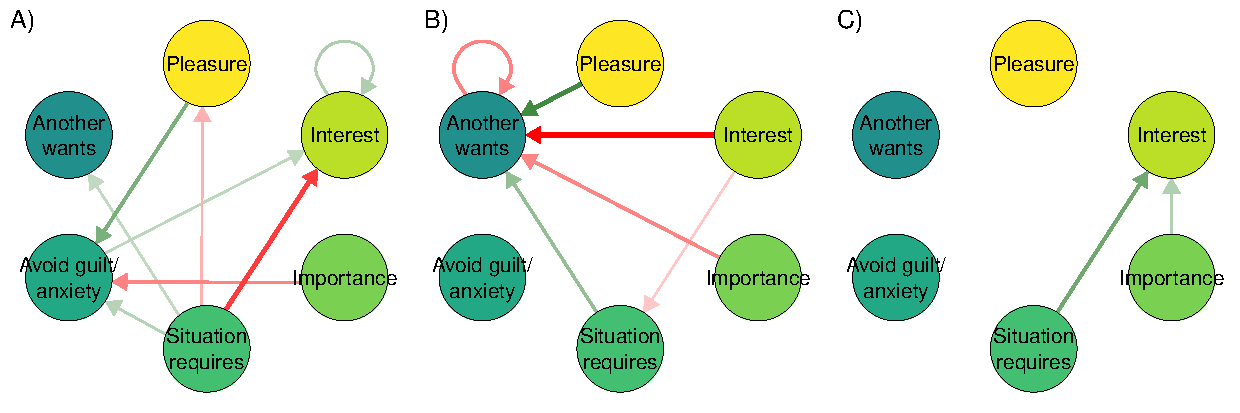
\includegraphics{_complexity-manuscript_files/figure-latex/tv-var-1.pdf}
\caption{\label{fig:tv-var}Relationships of a single participant's motivational variables varying in time. Columns, from left to right: Networks represent relationships between variables around the time points where 10\% (panel A), 50\% (B) and 90\% (C) of the study had been completed. An arrow from one variable to the next means the former predicts the latter at the next time point; green for positive and red for negative correlation.}
\end{figure}

Idiographic science, which tries to unveil person-level processes, does not aim to inductively go from data to universal or statistical laws which hold in hypothetical infinitely large populations (Gayles \& Molenaar, 2013). Instead, it applies general principles, such as universal properties of complex systems, to study how specific individuals behave in their particular contexts. Answering more than half a century of calls to expand focus beyond outcomes to processes, new technology in data collection and analysis have now made the idiographic approach possible (Hamaker et al., 2016). The basic solution is to not average individuals and then model behaviour of the averages, but to first model individuals, then aggregate those models to search for commonalities (Wright \& Woods, 2020). Recent work has made use of methods such as ecological momentary assessment (e.g.~Burke et al. (2017)) to gather time-series data on behaviour and determinants from one or more individuals over time. In the case of smoking, analyses of such idiographic data have yielded individualized models which can predict behaviour with stunning accuracy (for some individuals at least; Fisher and Soyster (2019); Soyster and Fisher (2019)).

Coming back to the notion of mechanisms; if the mechanisms happen within an individual, we need to study them at the appropriate scale, that is, within-individual. However, when we study individual time series data, it becomes quickly obvious that the methods used in the conventional approach for studying group averages (e.g.~pre-post measurements with a long time between them) leave us wanting. Figure \ref{fig:sampling-rate-plot} illustrates that if insufficient within-individual time points are sampled, a deceptively linear picture of the process emerges (see also Schiepek et al. (2016), p.~3). The same logic applies if we are studying groups but cannot rely on the means being informative due to a lack of power (as demonstrated in Carello and Moreno (2005)).

\begin{figure}
\centering
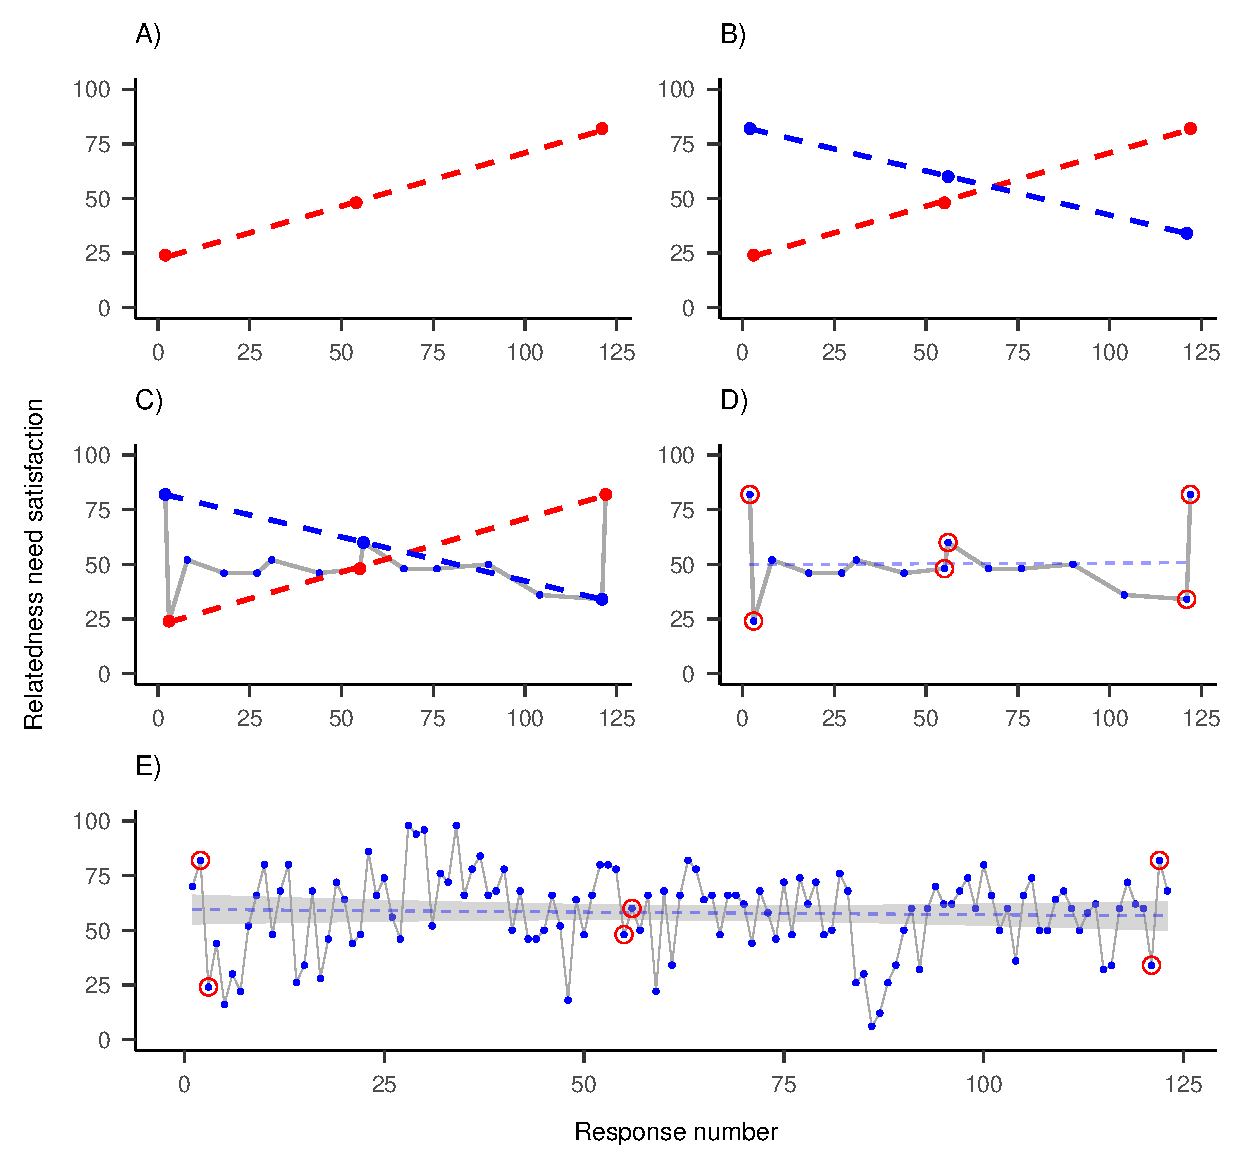
\includegraphics{_complexity-manuscript_files/figure-latex/sampling-rate-plot-1.pdf}
\caption{\label{fig:sampling-rate-plot}One of the time series collected by the participant featured in previous figure. Dots indicate answers to a visual analog scale question on their relatedness need satisfaction, as posited by self-determination theory (y-axis), measured on different time points (x-axis). A) Measuring three time points---representing conventional evaluation of baseline, post-intervention and a longer-term follow-up---shows a decreasing trend. B) Same measurement on slightly different days shows an opposite trend. C) Measuring 15 time points instead of three would have accommodated both observed \enquote{trends}. D) New linear regression line (dashed) indicates very slight upward trend. E) Including all of the 122 time points, a more complete picture of the dynamics emerges.}
\end{figure}

In sum, to study individual behaviour change, we need to not only collect intensive longitudinal data on the individual-level, but we must also consider the time evolution of the phenomenon and apply statistical analyses which can accurately model non-stationary data.

\hypertarget{nonlinear-dynamics}{%
\subsection{Nonlinear dynamics}\label{nonlinear-dynamics}}

As mentioned above, the linear methods traditionally used in psychology (e.g., multiple linear regression, ANOVA, and other cases of the general linear model) view psychological phenomena as following benign gradual changes over time. While sometimes useful as approximations, the assumptions of linear models are usually violated in practice (Siegenfeld \& Bar-Yam, 2019). Furthermore, linear models may be invalid when ceiling or floor effects are present (Verboon \& Peters, 2017; González, Coenders, Saez, \& Casas, 2010), or under \emph{hysterisis}, when the temporal direction of a relationship matters for its impact (e.g.~prevention is important precisely because it takes more effort to exit the state of having a lifestyle disease, than to enter it). Nonlinear growth can be very useful but unintuitive to grasp, as the world disovered during the COVID-19 pandemic: An multiplicative process with a doubling time of 3 days, starting from 10 cases, can lead to 10k cases by day 30 and well over 300 000 cases by day 45.

Theories and methods to understand non-linear change phenomena can provide to different types of answers than linear analyses. The most important factors in predicting behaviour change may not be the strength of a variable's relationship with behaviour (e.g.~regression weights), but rather the type of fluctuation that the variable exhibits in response to intervention (e.g.~so-called fractal, power-law, or 1/f noise; Bak et al. (1987), Almurad et al. (2018), and Delignieres et al. (2004)), or how fast it recovers from shocks (Van Orden et al., 2011). Another key insight is, that while we cannot usually predict in the sense of knowing what the value of the next observation will be, we can predict which system states are possible, and evaluate risks and opportunities for intervention from there.

Polynomial regression is perhaps the most commonly used model when linearity is questioned. This method allows for identifying curves that may better fit data on the relationships between variables than a straight line (e.g.~the convex (upward-curving) relationship demonstrated between intentions and behaviour between individuals; Chatzisarantis et al. (2019)), and can also be used to represent non-linear changes that occur over time. Polynomial regression models do not, however, adequately capture the essence of complex systems; nonlinear, irregular changes, periodic peaks and plateaus, and with recoveries after negative shocks and deterioration after positive ones (Hofmans et al., 2017, p. 2).

When we consider the situation where all components of a system interact, many features evident in everyday life but ambiguous in linear modelling become salient. Long periods with no discernible changes in outcomes might be followed by short bursts with large shifts. For example, a person's conscious intention to smoke may remain stable, while social norms keep changing, until one day a seemingly innocuous event causes the person to quit. When a system finally reaches a \enquote{tipping point} (e.g.~an individual's behaviour changes), conventional analytic methods have difficulty determining whether the effect was caused by a critically important incident, or by less obvious, small, cumulative effects over time which preceded the so-called \emph{phase transition}. Obviously, in such situations, the consequences of an incident (i.e.~breaking of the camel's back) do not relate linearly to the intensity of the event (i.e.~loading the last straw on the camel). This is a common dynamic in complex systems (Taleb \& Blyth, 2011), but it is extremely difficult to evaluate if information regarding the system is only available for a few points in time.

\hypertarget{empirical-solutions}{%
\section{Empirical solutions}\label{empirical-solutions}}

To model intensive longitudinal data, models developed within the literature on time series analysis (Bradley \& Kantz, 2015; Wright \& Woods, 2020) are necessary. A comprehensive contemporary treatment of individualised models is presented in. A time series in this case is a sequence of values representing one variable in one individual, and time series analysis consists of methods for studying ethe evolution of one or more time series.

The most common modelling framework, lag-1 autoregression, uses one previous time point as input to predicting the next one. In behavioural science, vector autoregression---vectors being sequences of numbers, representing values of variables---is often used to test the effects of several variables on the outcome of interest. One drawback of such autoregressive models is that they assume that there exists an average value around which the process fluctuates, which also motivates the common practice of \enquote{detrending}. In detrending, the researcher transforms the data by fitting a linear regression line and continuing the analysis with the residuals, often not taking into account that there can be several trends in subsections of the data (i.e.~the trend is non-stationary), which all contribute to what the linear model interprets as normally distributed \enquote{errors}. Moreover, the supposed mean value---as well as variance around it---may not remain the same across time (i.e.~the level is stationary), and the impact of previous time points on future ones is assumed to remain constant (Bringmann et al., 2017, p.~5). One way to overcome this particular shortcoming, is to let the parameters in autoregressive models vary across time, leading to the time-varying autoregressive model depicted in Figure \ref{fig:tv-var}. But we are still operating under the linear regression framework, with many of the accompanying assumptions, such as normally distributed errors. Furthermore, in Figure \ref{fig:tv-var} we have limited ourselves to investigating the lag-1 relationships, whereas long-range dependencies are common in complex systems.

How do we know if regression-based approaches are appropriate? The dynamics of all the variables in the model must conform to the required assumptions. The empirical researcher also has a wide variety of tests in his disposal. In the supplementary website (section xxx), we present a plethora of assumption tests, applied to a sample of 20 individuals collecting motivation data for nine variables. We can see that many variables indeed seem to exhibit non-stationary trends and levels, as well as non-linearities. Also, longer time series reject more of the assumptions, as the deviations from assumptions are not necessarily present in small samples, and larger samples confer higher statistical power. This does not, of course, give impetus to the suggestion that we ought to only gather short time series, as it would only mean we are not able to detect the deviations from assumptions, and our what we learn from the sample may not apply outside it.

There are many ways to study nonlinear change processes in complex systems. Behavioural researchers may find the generalised logistic model (Verboon \& Peters, 2017) a good starting point: This method produces readily-interpretable parameters indicating the floors and ceilings of the variables intervened upon, as well as the growth rate and timing of changes. Researchers may also be interested in identifying critical transformations taking place in a system (e.g.~a person's motivational system): In complex systems, these shifts may be preceded by warning signs such as increased turbulence (quantified as e.g.~\emph{dynamic complexity}; Schiepek and Strunk (2010)), or critical slowing down, i.e.~heightened autocorrelations in a time series, before (re)lapses occur (Leemput et al., 2014; Wichers et al., 2016). In clinical psychology interventions, intensive monitoring of psychopathological symptoms have allowed researchers to examine symptoms' variability, autocorrelations and other indicators of dynamics, and this has yielded considerable advances in the prediction of phase transitions between adaptive and maladaptive states during interventions ({\textbf{???}}; Olthof, Hasselman, Strunk, Aas, et al., 2019; Olthof, Hasselman, Strunk, van Rooij, et al., 2019). For example, Olthof et al.~(2019) identified that the presence of critical fluctuations was a key indicator of the effectiveness of psychotherapy for mood disorders. In the next section, we exemplify one particular family of analysis methods, recurrence quantification, due to its suitability for analysing many existing longitudinal data sets from a perspective with less a priori assumptions.

\hypertarget{modeling-complex-time-series-data-with-recurrence-quantification-analysis}{%
\subsection{Modeling complex time series data with recurrence quantification analysis}\label{modeling-complex-time-series-data-with-recurrence-quantification-analysis}}

To explore the dynamics of a phenomenon while making no assumptions about distributional shapes of observations or their errors, linearity, or time-lags involved, researchers can perform recurrence quantification analysis, which provides a visual intuition about the organisation of a system (recall from Table 1 that in complex systems, the organisation of components can be more important than the components themselves). Recurrence quantification analysis originates from physics (Marwan et al., 2007), but has been applied to a wide variety of fields in psychology (Brick et al., 2018; Navarro \& Arrieta, 2010; Rosen et al., 2013).

In recurrence plots, the re-occurrence of values is visualised by plotting a time series against another time series (to explore cross-recurrence) or itself (to explore auto-recurrence). Figure \ref{fig:rqa-pedagogical} depicts a cross-recurrence plot of two hypothetical time series with discrete states coded as 1 to 6: Yellow (1, 5, 4, 3, 2, 6) and Blue (5, 4, 3, 4, 3, 2). Black cells indicate places where the same value occurs in both series. These data show a switch in the system state: the blue series precedes the yellow one until time 3-4, after which the yellow series precedes the blue one. While this is merely a pedagogical example (a time series of only six observations would rarely be sufficient to reliably identify patterns), it illustrates the utility of the method in identifying patterns in time series data.

\begin{figure}
\centering
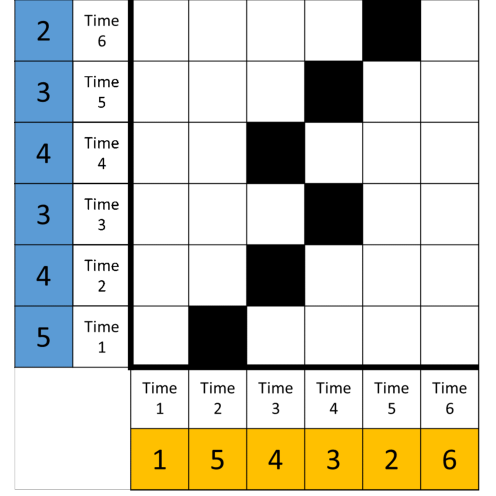
\includegraphics{_complexity-manuscript_files/figure-latex/rqa-pedagogical-1.pdf}
\caption{\label{fig:rqa-pedagogical}A recurrence plot of two hypothetical time series (blue and yellow) of length 6. We can observe, for example, that the blue series happens before the yellow one until a switch at time points 3-4, after which the yellow series leads.}
\end{figure}

Figure \ref{fig:rqa-multiplot} shows several auto-recurrence plots that depict longer time series of continuous data. Plots in the upper row colour cells based on the Euclidean distance between points of the underlying time series, with red colours indicating more similar values, blue colours less similar values, and white implying intermediate distance. For plots in the bottom row, a radius has been set to dichotomise each cell into \enquote{recurrent or not}, with the goal of creating a sparse matrix from which recurrences can be quantified (similar to that in Figure \ref{fig:rqa-pedagogical}). Because values always recur with themselves, we observe full recurrence in the diagonal line. The first column is a plot made out of a series of random numbers. The middle column depicts the result, where a single participant's responses on several motivation-related variables are subjected to multi-dimensional recurrence quantification analysis (Wallot, 2019; Wallot et al., 2016; Wallot \& Leonardi, 2018). The rightmost column represents surrogate data, where the participant's responses are shuffled to dismantle the temporal structure; this shuffling can be done repeatedly to produce confidence intervals for recurrence-based complexity measures.

In behaviour change research thus far, intensive longitudinal data have usually consisted of several variables, but not many (e.g.~\textless40) observations per variable. This is why we have omitted from describing a technique known as phase space reconstruction, which is commonly applied in recurrence quantification analysis, as it allows one to infer (topologically equivalent) dynamics of the multivariate system, from tracking one variable only (by what's known as Takens' theorem; Takens, 1981). The technique is explained in recurrence quantification primers (Coco \& Dale, 2014; Wallot \& Leonardi, 2018; Webber Jr \& Zbilut, 2005).

\begin{figure}
\centering
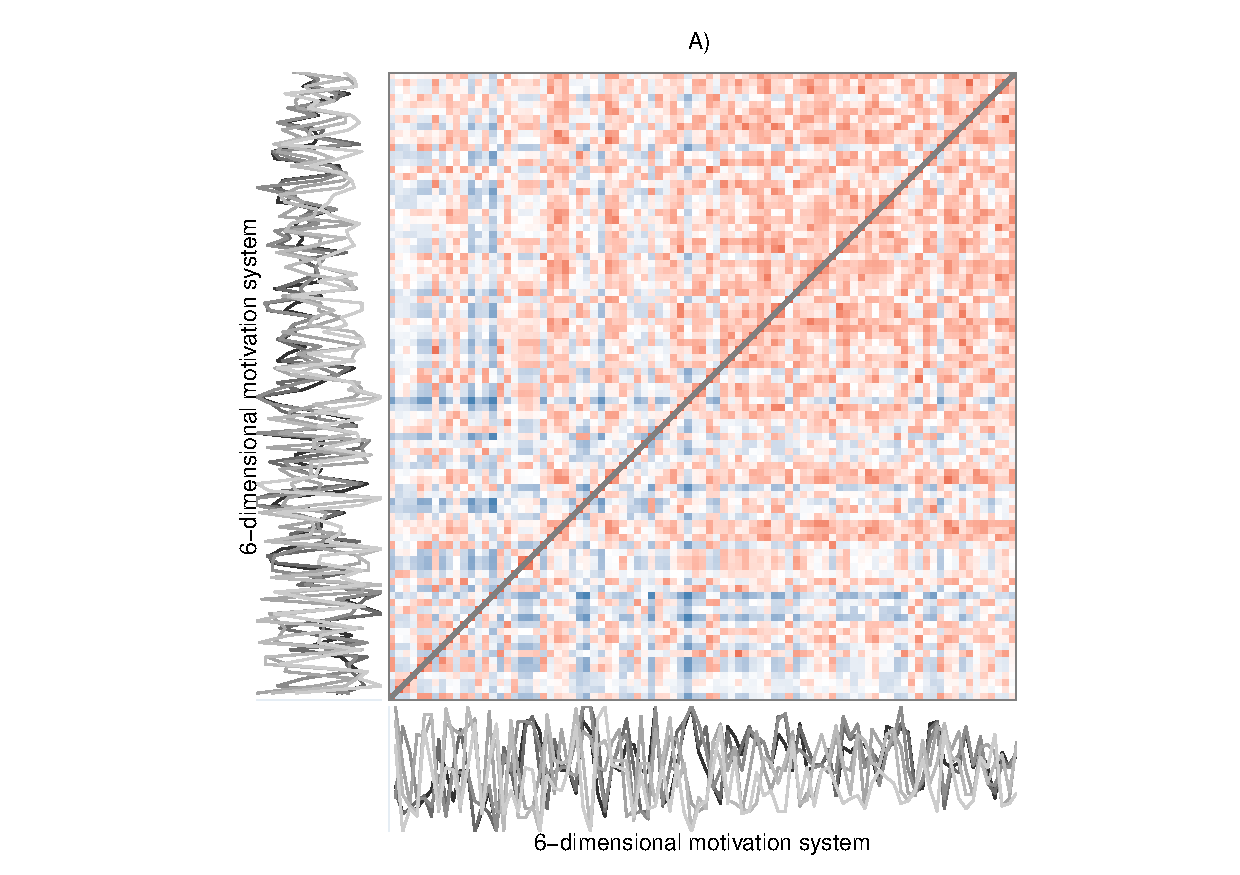
\includegraphics{_complexity-manuscript_files/figure-latex/rqa-multiplot-1.pdf}
\caption{\label{fig:rqa-multiplot}Recurrence plots. Columns, from left to right: Recurrence plots of uniformly distributed noise (A-B), a 6-dimensional motivation system of a single participant (C-D), and the same system with shuffled values (E-F). Panels A, C and E show unthresholded plots, where each cell represents a day, with red colours indicating the value is close to the corresponding time point on the other axis, while blue colours indicate the contrary. Panels B, D and F show matrices where these unthresholded plots have been binarised---leaving only 5\% of the closest points---leading to thresholded plots from which quantitative indicators can be calculated. Black points indicate the same or a similar value (in case of B) or configuration \enquote{profile} (in case of D and F) occurring. Drawn with R package casnet, code available at the supplementary website (section xxx).}
\end{figure}

It can be visually distinguished, that the middle column (panels C-D) of Figure \ref{fig:rqa-multiplot} has more structure than either the series of random numbers, or the series with shuffled numbers; the recurrent states mostly happen in the second half of the study period. There are also various ways to quantify the patterns in recurrence plots by extracting complexity measures from them. These metrics are somewhat beyond the scope of this paper, but fully described in Marwan, Romano, Thiel, \& Kurths ((2007), pp.~251 and 263-283). In the supplementary website (section xxx), we present a subset of them, which may be of particular interest to behaviour change researchers, with examples.

Recurrence plots are, in essence, visualisations of (Euclidean) distance matrices, and as such can also be represented as networks (Hasselman \& Bosman, 2020). This allows for displaying relationships between observations in the time series in an intuitive way, which in the case of multidimensional recurrence quantification analysis can be thought of displaying a type of multivariate \enquote{correlation}, indicating which occasions repeat a particular pattern. One such multidimensional recurrence network is demonstrated in Figure \ref{fig:recnet}. We can see that most of the recurrences take place in the second half of the data, as already shown in panels C and D of @ref(fig:rqa\_multiplot). In addition, all the 6-variable configurations which occur only once, take place in the first half of data collection.

\begin{figure}
\centering
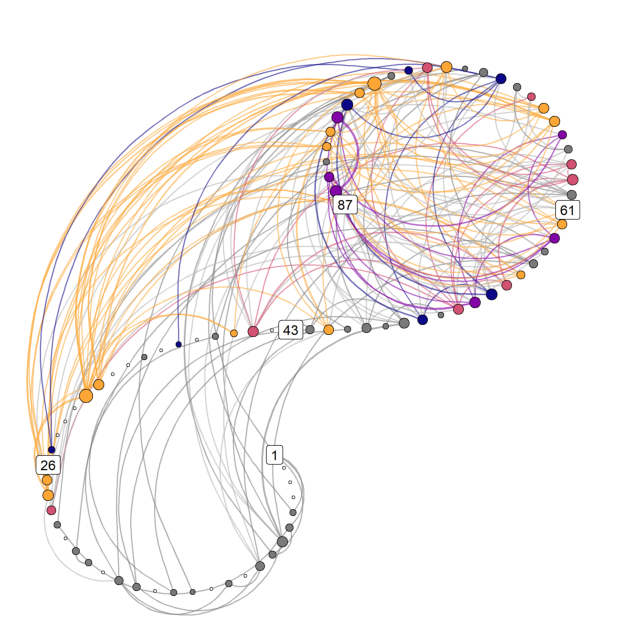
\includegraphics{_complexity-manuscript_files/figure-latex/recnet-1.pdf}
\caption{\label{fig:recnet}Recurrence network. Numbers indicate measurement occasions, and colors represent different motivation profiles, consisting of six variables, configurations of which can be conceived of as attractors. Lines indicate the same attractor reoccurring at a later time point. Yellow nodes indicate the strongest attractor, red nodes the second strongest, followed by purple and blue. Grey nodes depict uncategorised configurations which occur at least twice, and white ones the configurations, which only occur once. Nodes that are larger, are connected to more other nodes, especially those farther in time. Drawn with R package casnet, code available at the supplementary website (section xxx).}
\end{figure}

\hypertarget{discussion}{%
\section{Discussion}\label{discussion}}

Applied behavioural sciences, such as health psychology, have always studied phenomena like behaviour change mechanisms, which take place within complex ecological systems ({\textbf{???}}), but in the majority of cases we have tried to understand these phenomena using linear models, when the tools of complexity science would be more appropriate (Navarro et al., 2015). Behavioural scientists have an opportune moment to start considering complexity, as the field of behavioural intervention research is now taking committed first steps in this direction (Craig et al., 2018; Skivington et al., 2018), and there is a growing interest toward intervention programme theories that explicitly model complex aspects, such as recursive causality, disproportionate relationships, \enquote{tipping points}, and emergent outcomes (e.g.~Rogers, 2008). In addition, analytical methods that are compatible with complexity science, have recently been, and are increasingly being, developed ({\textbf{???}}).

Critically appraising the often hidden assumptions of models, especially in the context of complex systems such as human behaviour change interventions, is necessary for understanding the phenomena of interest and building a credible science. While researchers who study stable phenomena and only wish to draw group-level inferences (e.g.~to select promising public health interventions) are probably best served with traditional parsimonious models, this is rarely the case for psychologists and behaviour change intervention researchers who wish to understand how behaviour changes. For theory to advance, assumptions need to be justified: We cannot conclude both that our models for empirical testing omit crucial facets of reality, and at the same time imply real-life consequences. It is our position that a more fruitful approach would be to model coupled processes with individual-level psychological data from intensive longitudinal designs using analyses which are are reasonably free from assumptions regarding independence, ergodicity and linearity. By studying what other sciences know about change processes in complex systems, and establishing as well as replicating studies of human behaviour change, researchers can work towards uncovering more general principles of behaviour change. As Molenaar (2007) has pointed out, \enquote{the set of person-specific time series models thus obtained then can in the next step be subjected to standard analysis of inter-individual variation in order to detect subsets of subjects who are homogeneous with respect to particular aspects of the dynamical laws concerned}. In other words, information obtained from individual-level studies can then possibly inform models of larger groups, leading to better (or at least more humble) social scientific theories (Smaldino, Calanchini, \& Pickett, 2014).

\hypertarget{limitations}{%
\section{Limitations}\label{limitations}}

The field of complexity science and aligned novel methods is fast-moving, with new developments always on the horizon. However, there remain many practical and methodological barriers to fully embracing the complexity perspective in behaviour change research. Many of these barriers relate to data collection. While the development of smartphones and an array of other devices for ambulatory assessment allow the convenient collection of intensive longitudinal data, there are few stable and user-friendly open source options. This has resulted in large variability in the data collection tools used to produce intensive longitudinal data ({\textbf{???}}). Ensuring good adherence to these forms of data collection can be a challenge for researchers. For participants, adapting to intensive assessment is a behaviour change in itself -- particularly if they are required to use a specific device or smartphone application.

Long time series can be time-consuming and effortful to collect. It also creates a much greater burden on participants than traditional questionnaires and few timepoints only. However, in behaviour change research and health psychology, much of the core research interests of our theories---influences on behaviours---have traditionally been subjective factors (e.g., sense of self-efficacy, motivations and motives, outcome expectancies), only---by definition---accessible via self-report. This presents an undeniable practical challenge. Interestingly, and perhaps surprisingly, hundreds of EMA observations have been acquired in a variety of fields from xxx to yyy (see e.g.~REFS). Still, it is important to note that noisy momentary assessment data such as this could be supplemented with observational, ethnographic or interview data (Boulton, Allen, \& Bowman, 2015), as well as unobtrusive sensor data which provides a continuous signal (e.g.~from accelerometers or skin conductance sensors).

A number of methodological challenges for the study of dynamic systems in behavioural science have been identified (Hamaker \& Wichers, 2017). These involve, but are not limited to, measurement reactivity, the optimal choice of measurement intervals, and measurement quality. To properly address measurement reactivity, it is necessary to know whether the anticipation of measurement or the self-monitoring process itself (or both) interact with the outcomes of interest. Choosing an optimal measurement interval requires knowing the timescale of the mechanisms underlying behaviour change, which is rarely well understood. As regards measurement quality, we still lack a comprehensive approach to developing and establishing the quality of momentary measures of psychological constructs. Ensuring the validity and reliability of these measures can be difficult due to the requirement to use few items, not to mention that the questionnaire scales are themselves bounded, whereas experience hardly is. One solution for this is to inspect change profiles of responses (Hasselman \& Bosman, 2020) instead of raw scores. This alleviates, to an extent, the possibility of sudden shifts of how a person conceives the relation between their internal states and the slider or ordinal scale to which they ought to be projected to, as well as the likely situation where each answer is made with previous answers in mind. Following the analogy of Taleb, Canetti, Kinda, Loukoianova \& Schmieder ({\textbf{???}}); \enquote{Using an inaccurate tape measure will give a false reading of a child's height {[}\ldots{]} However, if one uses the same tape measure over time, it will give a reliable test of whether the child is growing}.

\hypertarget{conclusion}{%
\section{Conclusion}\label{conclusion}}

When a study finds that variables have explained an unsatisfactory proportion of behaviour, researchers often follow the pattern seen in social and organisational sciences and conclude that either: \enquote{(a) significant, explanatory variables have been omitted from the study, (b) the measurement instrument is too imprecise and \enquote{rough}, or that (c) the random or stochastic part of the problem has overwhelmed the patterned part} (Mathews et al., 1999, p. 453). But if the result stems from a model that makes unfounded assumptions (e.g.~linearity, relevance of the average over other metrics), is it any wonder that it fails to satisfactorily describe reality? In this paper, we have attempted to show that many real-world dynamics of behaviour change are inadequately captured by our seminal modelling strategies, and that changes are needed to advance our understanding of behaviour and behaviour change processes.

\hypertarget{list-of-abbreviations}{%
\subsubsection{List of abbreviations}\label{list-of-abbreviations}}

\noindent 
PA = Physical activity\\
MVPA = Moderate-to-vigorous physical activity\\
SB = Sedentary behaviour\\
BCT = Behaviour change technique\\
Nur = Practical nurse\\
HRC = Hotel, restaurant and catering studies\\
BA = Business and administration\\
IT = Business information technology

\hypertarget{declarations}{%
\subsection{Declarations}\label{declarations}}

\hypertarget{acknowledgements}{%
\subsubsection{Acknowledgements}\label{acknowledgements}}

We would like to thank participating schools, their staff and students, as well as the numerous people who have helped in study design and data collection. We are also grateful to Frederik Aust for technical support in creating a reproducible manuscript, as well as Ruben Arslan in creating the codebook.

\hypertarget{disclosure-of-interest}{%
\subsubsection{Disclosure of interest}\label{disclosure-of-interest}}

The authors report no conflict of interest.

\hypertarget{authors-contributions}{%
\subsubsection{Authors' contributions}\label{authors-contributions}}

MH wrote the analysis code, including the full online supplement, formulated the initial draft of the manuscript and revised it in collaboration with all co-authors. TV was responsible for planning and analysing the PA and SB measured from data collected with accelerometer. RS and EIF provided expertise regarding the statistical analyses. KB, AH, AU, VA-S, TV, RS and NH contributed to planning of the trial design and data collection including the measures used. NH, with the study co-applicants, conceived of the study. NH acted as principal investigator of the research project. All authors read and approved the final manuscript.

\hypertarget{prior-versions}{%
\subsubsection{Prior versions}\label{prior-versions}}

A pre-print has been uploaded to PsyArxiv (DOI: 10.31234/osf.io/46rzm).

\hypertarget{funding}{%
\subsubsection{Funding}\label{funding}}

MH was supported by Academy of Finland (grant number 295765) and Ministry for Education and Culture, Sports Science projects (grant number OKM/81/626/2014). NH was supported by an Academy of Finland Research Fellowship (grant number 285283). The data were collected in a project funded by Ministry for Education and Culture, Sports Science projects (grant number OKM/81/626/2014).

\hypertarget{preregistration}{%
\subsubsection{Preregistration}\label{preregistration}}

Trial Registration Number: ISRCTN10979479. Registered retrospectively: 31.12.2015.

\hypertarget{data-materials-and-online-resources}{%
\subsubsection{Data, materials, and online resources}\label{data-materials-and-online-resources}}

The analysis data will be available at \url{https://osf.io/jn9ax/} after the anonymisation process has been completed by the end of 2019. All analyses and code are available at \url{https://git.io/fNHuf} (permalink at Heino and Sund (2019), GitHub repository at \url{https://git.io/fjIQ6}). The electronic questionnaire form is available at \url{https://git.io/fjIP5}.

\hypertarget{reporting}{%
\subsubsection{Reporting}\label{reporting}}

We report all data exclusions, all manipulations, and all measures in the study. Sample size determination is reported in Hankonen et al.~(2016).

\hypertarget{ethical-approval}{%
\subsubsection{Ethical approval}\label{ethical-approval}}

The research proposal was reviewed by the Ethics Committee for Gynaecology and Obstetrics, Pediatrics and Psychiatry of the Hospital District of Helsinki and Uusimaa (decision number 367/13/03/03/2014).

\newpage

\hypertarget{references}{%
\section{References}\label{references}}

\begingroup
\setlength{\parindent}{-0.5in}
\setlength{\leftskip}{0.5in}

\hypertarget{refs}{}
\leavevmode\hypertarget{ref-almuradComplexityMatchingRestoring2018}{}%
Almurad, Z. M. H., Roume, C., Blain, H., \& Delignières, D. (2018). Complexity Matching: Restoring the Complexity of Locomotion in Older People Through Arm-in-Arm Walking. \emph{Frontiers in Physiology}, \emph{9}. \url{https://doi.org/10.3389/fphys.2018.01766}

\leavevmode\hypertarget{ref-bakSelforganizedCriticalityExplanation1987}{}%
Bak, P., Tang, C., \& Wiesenfeld, K. (1987). Self-organized criticality: An explanation of the 1/f noise. \emph{Physical Review Letters}, \emph{59}(4), 381--384. \url{https://doi.org/10.1103/PhysRevLett.59.381}

\leavevmode\hypertarget{ref-banduraSocialFoundationsThought1986}{}%
Bandura, A. (1986). \emph{Social foundations of thought and action: A social cognitive theory}. Prentice-Hall, Inc.

\leavevmode\hypertarget{ref-barabasiNetworkScience2016}{}%
Barabási, A.-L. (2016). \emph{Network Science}. Cambridge University Press.

\leavevmode\hypertarget{ref-bar-yamConceptsSystem2018}{}%
Bar-Yam, Y. (2018). \emph{Concepts: System}. https://web.archive.org/web/20181009095010/http://necsi.edu/guide/concepts/system.html.

\leavevmode\hypertarget{ref-bar-yamMakingThingsWork2004}{}%
Bar-Yam, Y. (2004). \emph{Making things work: Solving complex problems in a complex world}. NECSI/Knowledge Press.

\leavevmode\hypertarget{ref-borsboomNetworkTheoryMental2017}{}%
Borsboom, D. (2017). A network theory of mental disorders. \emph{World Psychiatry}, \emph{16}(1), 5--13. \url{https://doi.org/10.1002/wps.20375}

\leavevmode\hypertarget{ref-bradleyNonlinearTimeseriesAnalysis2015}{}%
Bradley, E., \& Kantz, H. (2015). Nonlinear time-series analysis revisited. \emph{Chaos: An Interdisciplinary Journal of Nonlinear Science}, \emph{25}(9), 097610.

\leavevmode\hypertarget{ref-brandTailoringHealthyWorkplace2015}{}%
Brand, S. L., Fleming, L. E., \& Wyatt, K. M. (2015). Tailoring healthy workplace interventions to local healthcare settings: A complexity theory-informed workplace of well-being framework. \emph{The Scientific World Journal}, \emph{2015}.

\leavevmode\hypertarget{ref-brickRecurrenceQuantificationAnalysis2018}{}%
Brick, T. R., Gray, A. L., \& Staples, A. D. (2018). Recurrence Quantification for the Analysis of Coupled Processes in Aging. \emph{The Journals of Gerontology: Series B}, \emph{73}(1), 134--147. \url{https://doi.org/10.1093/geronb/gbx018}

\leavevmode\hypertarget{ref-bringmannDonBlameModel2018a}{}%
Bringmann, L. F., \& Eronen, M. I. (2018). Don't blame the model: Reconsidering the network approach to psychopathology. \emph{Psychological Review}, \emph{125}(4), 606--615. \url{https://doi.org/10.1037/rev0000108}

\leavevmode\hypertarget{ref-burkeEcologicalMomentaryAssessment2017}{}%
Burke, L. E., Shiffman, S., Music, E., Styn, M. A., Kriska, A., Smailagic, A., Siewiorek, D., Ewing, L. J., Chasens, E., French, B., Mancino, J., Mendez, D., Strollo, P., \& Rathbun, S. L. (2017). Ecological Momentary Assessment in Behavioral Research: Addressing Technological and Human Participant Challenges. \emph{Journal of Medical Internet Research}, \emph{19}(3). \url{https://doi.org/10.2196/jmir.7138}

\leavevmode\hypertarget{ref-carelloWhyNonlinearMethods2005}{}%
Carello, C., \& Moreno, M. (2005). Why nonlinear methods. In \emph{Tutorials in contemporary nonlinear methods for the behavioral sciences} (pp. 1--25).

\leavevmode\hypertarget{ref-careyBehaviorChangeTechniques2019}{}%
Carey, R. N., Connell, L. E., Johnston, M., Rothman, A. J., de Bruin, M., Kelly, M. P., \& Michie, S. (2019). Behavior Change Techniques and Their Mechanisms of Action: A Synthesis of Links Described in Published Intervention Literature. \emph{Annals of Behavioral Medicine}, \emph{53}(8), 693--707. \url{https://doi.org/10.1093/abm/kay078}

\leavevmode\hypertarget{ref-cepedaSeasonalityPhysicalActivity2018}{}%
Cepeda, M., Koolhaas, C. M., van Rooij, F. J. A., Tiemeier, H., Guxens, M., Franco, O. H., \& Schoufour, J. D. (2018). Seasonality of physical activity, sedentary behavior, and sleep in a middle-aged and elderly population: The Rotterdam study. \emph{Maturitas}, \emph{110}, 41--50. \url{https://doi.org/10.1016/j.maturitas.2018.01.016}

\leavevmode\hypertarget{ref-chatzisarantisRelationshipPhysicalActivity2019}{}%
Chatzisarantis, N. L. D., Yli-Piipari, S., Schriefer, L. S., Wang, D., Barkoukis, V., \& Hagger, M. S. (2019). Is the relationship between physical activity intentions and behaviour convex? A test across 13 studies. \emph{Psychology of Sport and Exercise}, \emph{43}, 114--122. \url{https://doi.org/10.1016/j.psychsport.2019.01.013}

\leavevmode\hypertarget{ref-cocoCrossrecurrenceQuantificationAnalysis2014}{}%
Coco, M. I., \& Dale, R. (2014). Cross-recurrence quantification analysis of categorical and continuous time series: An R package. \emph{Frontiers in Psychology}, \emph{5}. \url{https://doi.org/10.3389/fpsyg.2014.00510}

\leavevmode\hypertarget{ref-coleTestingMediationalModels2003}{}%
Cole, D. A., \& Maxwell, S. E. (2003). Testing mediational models with longitudinal data: Questions and tips in the use of structural equation modeling. \emph{Journal of Abnormal Psychology}, \emph{112}(4), 558--577. \url{https://doi.org/10.1037/0021-843X.112.4.558}

\leavevmode\hypertarget{ref-craigTakingAccountContext2018}{}%
Craig, P., Di Ruggiero, E., Frolich, K. L., Mykhalovskiy, E., White, M., Campbell, R., Cummins, S., Edwards, N., Hunt, K., \& Kee, F. (2018). \emph{Taking account of context in population health intervention research: Guidance for producers, users and funders of research}.

\leavevmode\hypertarget{ref-cramerMajorDepressionComplex2016}{}%
Cramer, A. O. J., van Borkulo, C. D., Giltay, E. J., van der Maas, H. L. J., Kendler, K. S., Scheffer, M., \& Borsboom, D. (2016). Major Depression as a Complex Dynamic System. \emph{PLoS ONE}, \emph{11}(12). \url{https://doi.org/10.1371/journal.pone.0167490}

\leavevmode\hypertarget{ref-delignieresFractalDynamicsSelfesteem2004}{}%
Delignieres, D., Fortes, M., \& Ninot, G. (2004). The fractal dynamics of self-esteem and physical self. \emph{Nonlinear Dynamics, Psychology, and Life Sciences}, \emph{8}, 479--510.

\leavevmode\hypertarget{ref-dishmanDeterminantsPhysicalActivity1985}{}%
Dishman, R. K., Sallis, J. F., \& Orenstein, D. R. (1985). The determinants of physical activity and exercise. \emph{Public Health Reports}, \emph{100}(2), 158--171.

\leavevmode\hypertarget{ref-dumithPhysicalActivityChange2011}{}%
Dumith, S. C., Gigante, D. P., Domingues, M. R., \& Kohl, H. W. (2011). Physical activity change during adolescence: A systematic review and a pooled analysis. \emph{International Journal of Epidemiology}, \emph{40}(3), 685--698. \url{https://doi.org/10.1093/ije/dyq272}

\leavevmode\hypertarget{ref-finkSocialDeterminantsPopulation2016}{}%
Fink, D. S., Keyes, K. M., \& Cerdá, M. (2016). Social Determinants of Population Health: A Systems Sciences Approach. \emph{Current Epidemiology Reports}, \emph{3}(1), 98--105. \url{https://doi.org/10.1007/s40471-016-0066-8}

\leavevmode\hypertarget{ref-fisherLackGrouptoindividualGeneralizability2018}{}%
Fisher, A. J., Medaglia, J. D., \& Jeronimus, B. F. (2018). Lack of group-to-individual generalizability is a threat to human subjects research. \emph{Proceedings of the National Academy of Sciences}, 201711978. \url{https://doi.org/10.1073/pnas.1711978115}

\leavevmode\hypertarget{ref-fisherGeneratingAccuratePersonalized2019}{}%
Fisher, A. J., \& Soyster, P. D. (2019). \emph{Generating Accurate Personalized Predictions of Future Behavior: A Smoking Exemplar} {[}Preprint{]}. PsyArXiv. \url{https://doi.org/10.31234/osf.io/e24v6}

\leavevmode\hypertarget{ref-gaylesUtilityPersonspecificAnalyses2013}{}%
Gayles, J. G., \& Molenaar, P. C. M. (2013). The utility of person-specific analyses for investigating developmental processes: An analytic primer on studying the individual. \emph{International Journal of Behavioral Development}, \emph{37}(6), 549--562. \url{https://doi.org/10.1177/0165025413504857}

\leavevmode\hypertarget{ref-gomersallComplexAdaptiveSystems2018}{}%
Gomersall, T. (2018). Complex adaptive systems: A new approach for understanding health practices. \emph{Health Psychology Review}, \emph{0}(ja), 1--34. \url{https://doi.org/10.1080/17437199.2018.1488603}

\leavevmode\hypertarget{ref-hamakerModelingBASDysregulation2016}{}%
Hamaker, E. L., Grasman, R. P. P. P., \& Kamphuis, J. H. (2016). Modeling BAS Dysregulation in Bipolar Disorder: Illustrating the Potential of Time Series Analysis. \emph{Assessment}, \emph{23}(4), 436--446. \url{https://doi.org/10.1177/1073191116632339}

\leavevmode\hypertarget{ref-hamakerNoTimePresent2017}{}%
Hamaker, E. L., \& Wichers, M. (2017). No Time Like the Present: Discovering the Hidden Dynamics in Intensive Longitudinal Data. \emph{Current Directions in Psychological Science}, \emph{26}(1), 10--15. \url{https://doi.org/10.1177/0963721416666518}

\leavevmode\hypertarget{ref-hankonenLetMoveIt2016}{}%
Hankonen, N., Heino, M. T. J., Araujo-Soares, V., Sniehotta, F. F., Sund, R., Vasankari, T., Absetz, P., Borodulin, K., Uutela, A., Lintunen, T., \& Haukkala, A. (2016). ``Let's Move It'' a school-based multilevel intervention to increase physical activity and reduce sedentary behaviour among older adolescents in vocational secondary schools: A study protocol for a cluster-randomised trial. \emph{BMC Public Health}, \emph{16}, 451--466. \url{https://doi.org/10.1186/s12889-016-3094-x}

\leavevmode\hypertarget{ref-hasselmanStudyingComplexAdaptive2020}{}%
Hasselman, F., \& Bosman, A. M. T. (2020). Studying Complex Adaptive Systems with Internal States: A Recurrence Network Approach to the Analysis of Multivariate Time Series Data Representing Self-Reports of Human Experience. \emph{Frontiers in Applied Mathematics and Statistics}, \emph{6}. \url{https://doi.org/10.3389/fams.2020.00009}

\leavevmode\hypertarget{ref-haweTheorisingInterventionsEvents2009}{}%
Hawe, P., Shiell, A., \& Riley, T. (2009). Theorising Interventions as Events in Systems. \emph{American Journal of Community Psychology}, \emph{43}(3-4), 267--276. \url{https://doi.org/10.1007/s10464-009-9229-9}

\leavevmode\hypertarget{ref-heinoVisualisationNetworkAnalysis2019a}{}%
Heino, M. T. J., Knittle, K., Fried, E., Sund, R., Haukkala, A., Borodulin, K., Uutela, A., Araujo-Soares, V., Vasankari, T., \& Hankonen, N. (2019). Visualisation and network analysis of physical activity and its determinants: Demonstrating opportunities in analysing baseline associations in the let's move it trial. \emph{Health Psychology and Behavioral Medicine}, \emph{7}(1), 269--289. \url{https://doi.org/10.1080/21642850.2019.1646136}

\leavevmode\hypertarget{ref-heinoSourceCodeVisualisation2019}{}%
Heino, M. T. J., \& Sund, R. (2019). \emph{Source code: Visualisation and network analysis of physical activity and its determinants}. Zenodo. \url{https://doi.org/10.5281/zenodo.2628764}

\leavevmode\hypertarget{ref-hofmansKCentresFunctionalClustering2017}{}%
Hofmans, J., Vantilborgh, T., \& Solinger, O. N. (2017). K-Centres Functional Clustering: A Person-Centered Approach to Modeling Complex Nonlinear Growth Trajectories. \emph{Organizational Research Methods}, 1094428117725793. \url{https://doi.org/10.1177/1094428117725793}

\leavevmode\hypertarget{ref-johnstonUsefulTheoriesShould2013}{}%
Johnston, D. W., \& Johnston, M. (2013). Useful theories should apply to individuals. \emph{British Journal of Health Psychology}, \emph{18}(3), 469--473. \url{https://doi.org/10.1111/bjhp.12049}

\leavevmode\hypertarget{ref-kokIgnoringTheoryMisinterpreting2018}{}%
Kok, G., Peters, G.-J. Y., Kessels, L. T., Ten Hoor, G. A., \& Ruiter, R. A. (2018). Ignoring theory and misinterpreting evidence: The false belief in fear appeals. \emph{Health Psychology Review}, \emph{12}(2), 111--125.

\leavevmode\hypertarget{ref-kwasnickaTheoreticalExplanationsMaintenance2016}{}%
Kwasnicka, D., Dombrowski, S. U., White, M., \& Sniehotta, F. (2016). Theoretical explanations for maintenance of behaviour change: A systematic review of behaviour theories. \emph{Health Psychology Review}, \emph{10}(3), 277--296. \url{https://doi.org/10.1080/17437199.2016.1151372}

\leavevmode\hypertarget{ref-leemputCriticalSlowingEarly2014}{}%
Leemput, I. A. van de, Wichers, M., Cramer, A. O. J., Borsboom, D., Tuerlinckx, F., Kuppens, P., Nes, E. H. van, Viechtbauer, W., Giltay, E. J., Aggen, S. H., Derom, C., Jacobs, N., Kendler, K. S., Maas, H. L. J. van der, Neale, M. C., Peeters, F., Thiery, E., Zachar, P., \& Scheffer, M. (2014). Critical slowing down as early warning for the onset and termination of depression. \emph{Proceedings of the National Academy of Sciences}, \emph{111}(1), 87--92. \url{https://doi.org/10.1073/pnas.1312114110}

\leavevmode\hypertarget{ref-makridakisForecastingSocialSettings2019}{}%
Makridakis, S., Hyndman, R. J., \& Petropoulos, F. (2019). Forecasting in social settings: The state of the art. \emph{International Journal of Forecasting}. \url{https://doi.org/10.1016/j.ijforecast.2019.05.011}

\leavevmode\hypertarget{ref-makridakisDecisionMakingPlanning2009}{}%
Makridakis, S., \& Taleb, N. (2009). Decision making and planning under low levels of predictability. \emph{International Journal of Forecasting}, \emph{25}(4), 716--733. \url{https://doi.org/10.1016/j.ijforecast.2009.05.013}

\leavevmode\hypertarget{ref-marwanRecurrencePlotsAnalysis2007}{}%
Marwan, N., Romano, M. C., Thiel, M., \& Kurths, J. (2007). Recurrence plots for the analysis of complex systems. \emph{Physics Reports}, \emph{438}(5), 237--329. \url{https://doi.org/10.1016/j.physrep.2006.11.001}

\leavevmode\hypertarget{ref-mathewsWhyStudyComplexity1999}{}%
Mathews, K. M., White, M. C., \& Long, R. G. (1999). Why Study the Complexity Sciences in the Social Sciences? \emph{Human Relations}, \emph{52}(4), 439--462. \url{https://doi.org/10.1177/001872679905200402}

\leavevmode\hypertarget{ref-matthewsSourcesVarianceDaily2002}{}%
Matthews, C. E., Ainsworth, B. E., Thompson, R. W., \& Bassett, D. R. (2002). Sources of variance in daily physical activity levels as measured by an accelerometer. \emph{Medicine and Science in Sports and Exercise}, \emph{34}(8), 1376--1381.

\leavevmode\hypertarget{ref-maySimpleMathematicalModels1976}{}%
May, R. M. (1976). Simple mathematical models with very complicated dynamics. \emph{Nature}, \emph{261}(5560), 459--467. \url{https://doi.org/10.1038/261459a0}

\leavevmode\hypertarget{ref-meehlWhySummariesResearch1990}{}%
Meehl, P. E. (1990). Why summaries of research on psychological theories are often uninterpretable. \emph{Psychological Reports}, \emph{66}(1), 195--244. \url{https://doi.org/10.2466/pr0.1990.66.1.195}

\leavevmode\hypertarget{ref-michieABCBehaviourChange2014}{}%
Michie, S., West, R., Campbell, R., Brown, J., \& Gainforth, H. (2014). \emph{ABC of behaviour change theories}.

\leavevmode\hypertarget{ref-mitchellComplexityGuidedTour2009}{}%
Mitchell, M. (2009). \emph{Complexity: A guided tour}. Oxford University Press.

\leavevmode\hypertarget{ref-molenaarNewPersonspecificParadigm2009}{}%
Molenaar, P. C., \& Campbell, C. G. (2009). The new person-specific paradigm in psychology. \emph{Current Directions in Psychological Science}, \emph{18}(2), 112--117.

\leavevmode\hypertarget{ref-molenaarImplicationsClassicalErgodic2008}{}%
Molenaar, P. C. M. (2008). On the implications of the classical ergodic theorems: Analysis of developmental processes has to focus on intra-individual variation. \emph{Developmental Psychobiology}, \emph{50}(1), 60--69. \url{https://doi.org/10.1002/dev.20262}

\leavevmode\hypertarget{ref-molenaarManifestoPsychologyIdiographic2004}{}%
Molenaar, P. C. M. (2004). A manifesto on psychology as idiographic science: Bringing the person back into scientific psychology, this time forever. \emph{Measurement}, \emph{2}(4), 201--218.

\leavevmode\hypertarget{ref-navarroChaosHumanBehavior2010}{}%
Navarro, J., \& Arrieta, C. (2010). Chaos in human behavior: The case of work motivation. \emph{The Spanish Journal of Psychology}, \emph{13}(1), 244--256.

\leavevmode\hypertarget{ref-navarroTakingTimeSeriously2015}{}%
Navarro, J., Roe, R. A., \& Artiles, M. I. (2015). Taking time seriously: Changing practices and perspectives in Work/Organizational Psychology. \emph{Revista de Psicología Del Trabajo Y de Las Organizaciones}, \emph{31}(3), 135--145. \url{https://doi.org/10.1016/j.rpto.2015.07.002}

\leavevmode\hypertarget{ref-navarroHealthyVariabilityOrganizational2015}{}%
Navarro, J., \& Rueff-Lopes, R. (2015). Healthy variability in organizational behavior: Empirical evidence and new steps for future research. \emph{Nonlinear Dynamics, Psychology, and Life Sciences}, \emph{19}(4), 529--552.

\leavevmode\hypertarget{ref-olthofDestabilizationSelfratingsPsychotherapeutic2019}{}%
Olthof, M., Hasselman, F., Strunk, G., Aas, B., Schiepek, G., \& Lichtwarck-Aschoff, A. (2019). Destabilization in self-ratings of the psychotherapeutic process is associated with better treatment outcome in patients with mood disorders. \emph{Psychotherapy Research}, \emph{0}(0), 1--12. \url{https://doi.org/10.1080/10503307.2019.1633484}

\leavevmode\hypertarget{ref-olthofCriticalFluctuationsEarlyWarning2019}{}%
Olthof, M., Hasselman, F., Strunk, G., van Rooij, M., Aas, B., Helmich, M. A., Schiepek, G., \& Lichtwarck-Aschoff, A. (2019). Critical Fluctuations as an Early-Warning Signal for Sudden Gains and Losses in Patients Receiving Psychotherapy for Mood Disorders. \emph{Clinical Psychological Science}, 2167702619865969. \url{https://doi.org/10.1177/2167702619865969}

\leavevmode\hypertarget{ref-petersPragmaticNihilismHow2017}{}%
Peters, G.-J. Y., \& Crutzen, R. (2017). Pragmatic nihilism: How a Theory of Nothing can help health psychology progress. \emph{Health Psychology Review}, \emph{11}(2), 103--121. \url{https://doi.org/10.1080/17437199.2017.1284015}

\leavevmode\hypertarget{ref-petersConsensusFearAppeals2018}{}%
Peters, G.-J. Y., Ruiter, R. A., Ten Hoor, G. A., Kessels, L. T., \& Kok, G. (2018). Towards consensus on fear appeals: A rejoinder to the commentaries on Kok, Peters, Kessels, ten Hoor, and Ruiter (2018). \emph{Health Psychology Review}, \emph{12}(2), 151--156.

\leavevmode\hypertarget{ref-resnicowChaoticViewBehavior2006}{}%
Resnicow, K., \& Vaughan, R. (2006). A chaotic view of behavior change: A quantum leap for health promotion. \emph{International Journal of Behavioral Nutrition and Physical Activity}, \emph{3}(1), 25. \url{https://doi.org/10.1186/1479-5868-3-25}

\leavevmode\hypertarget{ref-richardsonInteractionDominantDynamicsTimescale2017}{}%
Richardson, M. J., Kallen, R. W., \& Eiler, B. A. (2017). Interaction-Dominant Dynamics, Timescale Enslavement, and the Emergence of Social Behavior. In \emph{Computational Social Psychology} (pp. 121--142). Routledge.

\leavevmode\hypertarget{ref-ricklesCausalityComplexInterventions2009}{}%
Rickles, D. (2009). Causality in complex interventions. \emph{Medicine, Health Care, and Philosophy}, \emph{12}(1), 77--90. \url{https://doi.org/10.1007/s11019-008-9140-4}

\leavevmode\hypertarget{ref-ricklesSimpleGuideChaos2007}{}%
Rickles, D., Hawe, P., \& Shiell, A. (2007). A simple guide to chaos and complexity. \emph{Journal of Epidemiology \& Community Health}, \emph{61}(11), 933--937. \url{https://doi.org/10.1136/jech.2006.054254}

\leavevmode\hypertarget{ref-rosenKnowItWhen2013}{}%
Rosen, P. J., Epstein, J. N., \& Orden, G. V. (2013). I know it when I quantify it: Ecological momentary assessment and recurrence quantification analysis of emotion dysregulation in children with ADHD. \emph{ADHD Attention Deficit and Hyperactivity Disorders}, \emph{5}(3), 283--294. \url{https://doi.org/10.1007/s12402-013-0101-2}

\leavevmode\hypertarget{ref-schiepekRealtimeMonitoringPsychotherapeutic2016}{}%
Schiepek, G., Aichhorn, W., Gruber, M., Strunk, G., Bachler, E., \& Aas, B. (2016). Real-time monitoring of psychotherapeutic processes: Concept and compliance. \emph{Frontiers in Psychology}, \emph{7}, 604.

\leavevmode\hypertarget{ref-schiepekIdentificationCriticalFluctuations2010}{}%
Schiepek, G., \& Strunk, G. (2010). The identification of critical fluctuations and phase transitions in short term and coarse-grained time seriesa method for the real-time monitoring of human change processes. \emph{Biological Cybernetics}, \emph{102}(3), 197--207. \url{https://doi.org/10.1007/s00422-009-0362-1}

\leavevmode\hypertarget{ref-siegenfeldIntroductionComplexSystems2019}{}%
Siegenfeld, A. F., \& Bar-Yam, Y. (2019). An Introduction to Complex Systems Science and its Applications. \emph{arXiv:1912.05088 {[}Physics{]}}. \url{http://arxiv.org/abs/1912.05088}

\leavevmode\hypertarget{ref-skivingtonDevelopingEvaluatingComplex2018}{}%
Skivington, K., Matthews, L., Craig, P., Simpson, S., \& Moore, L. (2018). Developing and evaluating complex interventions: Updating Medical Research Council guidance to take account of new methodological and theoretical approaches. \emph{The Lancet}, \emph{392}, S2. \url{https://doi.org/10.1016/S0140-6736(18)32865-4}

\leavevmode\hypertarget{ref-soysterInvolvingStakeholdersDesign2019}{}%
Soyster, P. D., \& Fisher, A. J. (2019). Involving stakeholders in the design of ecological momentary assessment research: An example from smoking cessation. \emph{PLOS ONE}, \emph{14}(5), e0217150. \url{https://doi.org/10.1371/journal.pone.0217150}

\leavevmode\hypertarget{ref-strogatzNonlinearDynamicsChaos2018}{}%
Strogatz, S. H. (2018). \emph{Nonlinear Dynamics and Chaos: With Applications to Physics, Biology, Chemistry, and Engineering}.

\leavevmode\hypertarget{ref-talebAntifragilityMathematicalIdea2013}{}%
Taleb, N. N. (2013). 'Antifragility' as a mathematical idea. \emph{Nature}, \emph{494}(7438), 430--430. \url{https://doi.org/10.1038/494430e}

\leavevmode\hypertarget{ref-talebAntifragileThingsThat2012}{}%
Taleb, N. N. (2012). \emph{Antifragile: Things that gain from disorder} (1st ed). Random House.

\leavevmode\hypertarget{ref-talebBlackSwanCairo2011}{}%
Taleb, N. N., \& Blyth, M. (2011). The Black Swan of Cairo. \emph{Foreign Affairs}.

\leavevmode\hypertarget{ref-vanordenLivingPinkIntentionality2011}{}%
Van Orden, G. C., Kloos, H., \& Wallot, S. (2011). Living in the Pink: Intentionality, Wellbeing, and Complexity. In C. Hooker (Ed.), \emph{Philosophy of Complex Systems} (Vol. 10, pp. 629--672). North-Holland. \url{https://doi.org/10.1016/B978-0-444-52076-0.50022-5}

\leavevmode\hypertarget{ref-wallotMultidimensionalCrossRecurrenceQuantification2019}{}%
Wallot, S. (2019). Multidimensional Cross-Recurrence Quantification Analysis (MdCRQA) A Method for Quantifying Correlation between Multivariate Time-Series. \emph{Multivariate Behavioral Research}, \emph{54}(2), 173--191. \url{https://doi.org/10.1080/00273171.2018.1512846}

\leavevmode\hypertarget{ref-wallotInteractionDominantCausationMind2017}{}%
Wallot, S., \& Kelty-Stephen, D. G. (2017). Interaction-Dominant Causation in Mind and Brain, and Its Implication for Questions of Generalization and Replication. \emph{Minds and Machines}, 1--22. \url{https://doi.org/10.1007/s11023-017-9455-0}

\leavevmode\hypertarget{ref-wallotAnalyzingMultivariateDynamics2018}{}%
Wallot, S., \& Leonardi, G. (2018). Analyzing Multivariate Dynamics Using Cross-Recurrence Quantification Analysis (CRQA), Diagonal-Cross-Recurrence Profiles (DCRP), and Multidimensional Recurrence Quantification Analysis (MdRQA) A Tutorial in R. \emph{Frontiers in Psychology}, \emph{9}. \url{https://doi.org/10.3389/fpsyg.2018.02232}

\leavevmode\hypertarget{ref-wallotMultidimensionalRecurrenceQuantification2016}{}%
Wallot, S., Roepstorff, A., \& Mønster, D. (2016). Multidimensional Recurrence Quantification Analysis (MdRQA) for the Analysis of Multidimensional Time-Series: A Software Implementation in MATLAB and Its Application to Group-Level Data in Joint Action. \emph{Frontiers in Psychology}, \emph{7}. \url{https://doi.org/10.3389/fpsyg.2016.01835}

\leavevmode\hypertarget{ref-webberjrRecurrenceQuantificationAnalysis2005}{}%
Webber Jr, C. L., \& Zbilut, J. P. (2005). Recurrence quantification analysis of nonlinear dynamical systems. In \emph{Tutorials in contemporary nonlinear methods for the behavioral sciences} (pp. 26--94).

\leavevmode\hypertarget{ref-westHomeostasisGaussStatistics2010}{}%
West, B. J. (2010). Homeostasis and Gauss statistics: Barriers to understanding natural variability: Homeostasis and Gauss statistics. \emph{Journal of Evaluation in Clinical Practice}, \emph{16}(3), 403--408. \url{https://doi.org/10.1111/j.1365-2753.2010.01459.x}

\leavevmode\hypertarget{ref-westScaleUniversalLaws2017}{}%
West, G. (2017). \emph{Scale: The Universal Laws of Growth, Innovation, Sustainability, and the Pace of Life in Organisms, Cities, Economies, and Companies} (1st ed.). Penguin Press.

\leavevmode\hypertarget{ref-wichersCriticalSlowingPersonalized2016}{}%
Wichers, M., Groot, P. C., \& Psychosystems, E. G. (2016). Critical Slowing Down as a Personalized Early Warning Signal for Depression. \emph{Psychotherapy and Psychosomatics}, \emph{85}(2), 114--116. \url{https://doi.org/10.1159/000441458}

\leavevmode\hypertarget{ref-wrightPersonalizedModelsPsychopathology2020a}{}%
Wright, A. G. C., \& Woods, W. C. (2020). Personalized Models of Psychopathology. \emph{Annual Review of Clinical Psychology}, \emph{16}(1). \url{https://doi.org/10.1146/annurev-clinpsy-102419-125032}

\leavevmode\hypertarget{ref-wrightThinkingSystemsPrimer2009}{}%
Wright, D., \& Meadows, D. H. (2009). \emph{Thinking in Systems: A Primer} (First edition). Routledge.

\leavevmode\hypertarget{ref-zhangSocialNetworksHealth2019}{}%
Zhang, J., \& Centola, D. (2019). Social Networks and Health: New Developments in Diffusion, Online and Offline. \emph{Annual Review of Sociology}, \emph{45}(1), 91--109. \url{https://doi.org/10.1146/annurev-soc-073117-041421}

\endgroup

\end{document}
